\documentclass[12pt,a4paper]{scrreprt}
 
\usepackage[german]{babel}
\usepackage[utf8]{inputenc}
\usepackage[T1]{fontenc}
\usepackage{ae}
\usepackage[bookmarks,bookmarksnumbered]{hyperref}
\usepackage{graphicx}
\usepackage{floatflt}
\usepackage{enumitem}
\usepackage{pifont}
\setlength{\parindent}{0pt}
 
\begin{document}

\title{Anwenderdokumentation}
\subtitle{ILIAS Review Plugin}
\publishers{Version: 5.0, Status: Fertiggestellt}
\author{SWT-Gruppe 04\\ \\Auftraggeber: Thordis Kombrink\\Weitere: Dr Birgit Demuth, Professor Wollersheim\\Tutor: Andy P"uschel}
\maketitle
\tableofcontents

\chapter{Willkommen}
Herzlich Willkommen zur Anwenderdokumentation des Review-Plugins für das OpenSource Lernsystem ILIAS der Gruppe 4, entwickelt im Wintersemester 2014/2015. Vielen Dank, dass Sie sich für unser Plugin interessieren. Die folgenden Seiten sollen Ihnen helfen, die Software kennen zu lernen und effektiv zu nutzen. 

\section{Grundsätze dieser Dokumentation}
Diese Dokumentation beschreibt nur die Funktionalitäten, die das Team selbst bereit stellt, um ein Reviewplugin für ILIAS zu ermöglichen. Informationen zur Installation von ILIAS, zu dessen Handhabung und standardmäßig ILIAS-eigene Funktionalitäten sind in der umfassenden Benutzerdokumentation
\footnote{\label{foot:1}http://www.ilias.de/docu/goto\_docu\_cat\_3866.html} von ILIAS nachzulesen. 

\section{Einrichtung der Software}
Zum Betreiben des Plugins bedarf es eines Webservers, auf dem ILIAS in der Version 4.4.5, MySQL in der Version 5.0.11 und PHP in der Version 5.5.11 bereits vollständig installiert ist. Es ist möglich, dass das Review-Plugin auch mit abweichenden Versionen einwandfrei zu benutzen ist.
Zur Installation müssen 2 Pakete heruntergeladen werden: assReviewableMultipleChoice\footnote{\label{foot:2}https://github.com/daelmo/assReviewableMultipleChoice}	und Review
\footnote{\label{foot:3}https://github.com/daelmo/Review}. 
	assReviewableMultipleChoice muss auf dem Webserver in das Verzeichnis ilias/Customizing/global/plugins/ Modules/TestQuestionPool/Questions/ entpackt werden. Review wird hingegen in /ilias/Customizing/global/plugins/Services/Repository/RepositoryObject/ entpackt.
	Beide Pakete sind voneinander abhängig und es bedarf beider Pakete um das Plugin nutzen zu können.
	
\section{Der erste Start}
Der Administrator des installierten ILIAS-Systems muss beide Plugins aktivieren. Dazu ist seine Anmeldung in ILIAS notwendig. Unter Administration findet er den Link 'Plugins'. Auf der verlinkten Seite werden alle vorhandenen Plugins angezeigt. Es ist notwendig, dass er Review und assReviewableMultipleChoice aktualisiert und zulässt. \\
	Um das Plugin in einer Gruppe zum Reviewen von Fragen nutzen zu können, muss in der Gruppe ein Fragenpool angelegt sein. Desweiteren muss nun ein Reviewpool angelegt werden.\\
	Es ist möglich mehrere Fragenpools oder auch Reviewpools zu erstellen, doch ist dies bei Reviewpools nicht sinnvoll. 

\chapter{Struktur}

\section{Erstellungsseite der Fragen}
Die Seite trifft man im Fragenpool an, wenn eine neue reviewbare Frage erstellt werden soll. Sie sieht der Seite zum Erstellen einfacher Multiple Choice-Fragen sehr ähnlich. Zusätzlich gibt der Nutzer nur den kognitiven Prozess an, sowie die Wissensdimension, in die er die Frage einordnet. Dafür sind zwei Auswahlfelder im unteren Teil des Formulars vorgesehen.\\
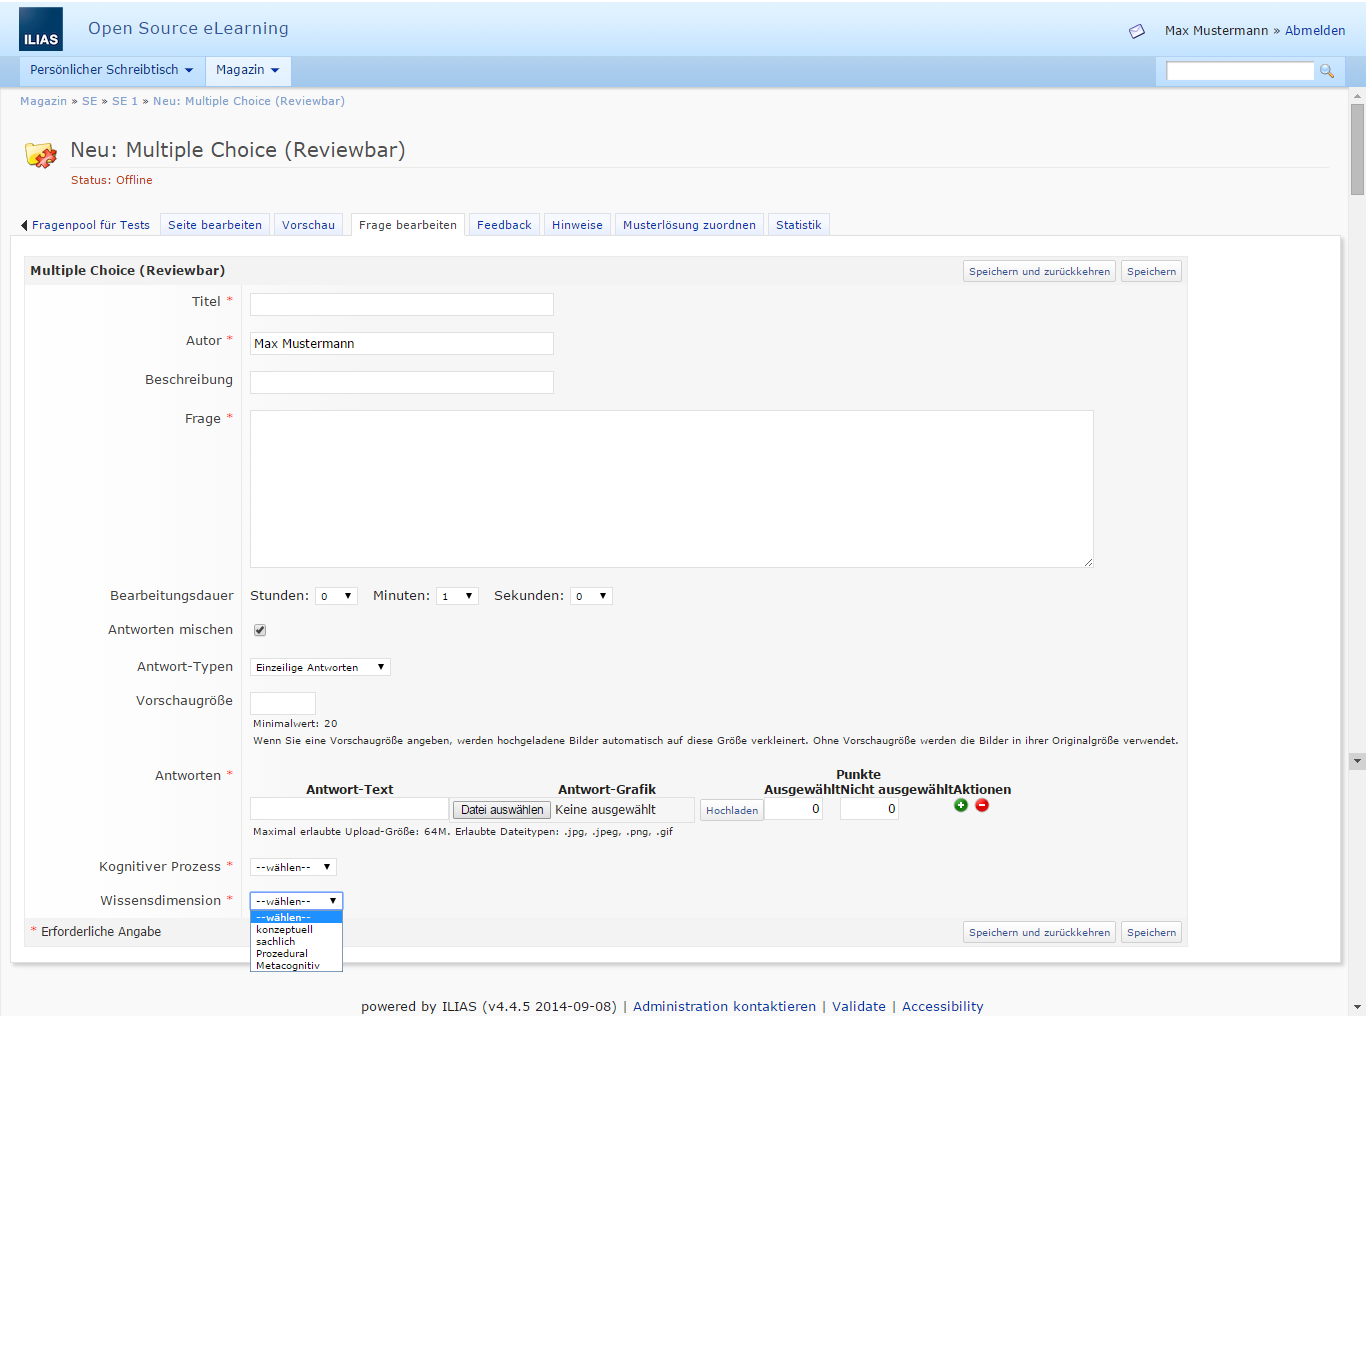
\includegraphics[width=0.9\textwidth]{frage_erstellen.png}
\\
\section{eigene \"Ubersichtsseite}
In jedem Reviewpool findet der Nutzer als erstes eine Übersicht in Form von zwei Tabellen an, mit der er einen Überblick über von ihm erstellte Fragen, die zurzeit reviewt werden, sowie seine bereits geschriebenen und noch ausstehenden Reviews erhält. 	

\section{Erstellungsseite der Reviews}
Beim Erstellen eines Reviews erhält man eine Übersicht über die Frage, die reviewt werden soll, dabei ist der Ersteller der Frage anonym. Allein der Administrator kann diesen einsehen.
Auf die Frage folgt das Review-Eingabeformular mit einer Reihe von Checkboxen die ausgefüllt werden müssen um die erstellte Frage einzuschätzen. Es wird eine schriftliche Bemerkung verlangt, warum die Frage akzeptiert, abgelehnt wird oder überarbeitet werden muss.
Anschließend wird die selbst eingeschätzte Expertise angegeben und das Review kann abgesendet werden.\\
\\
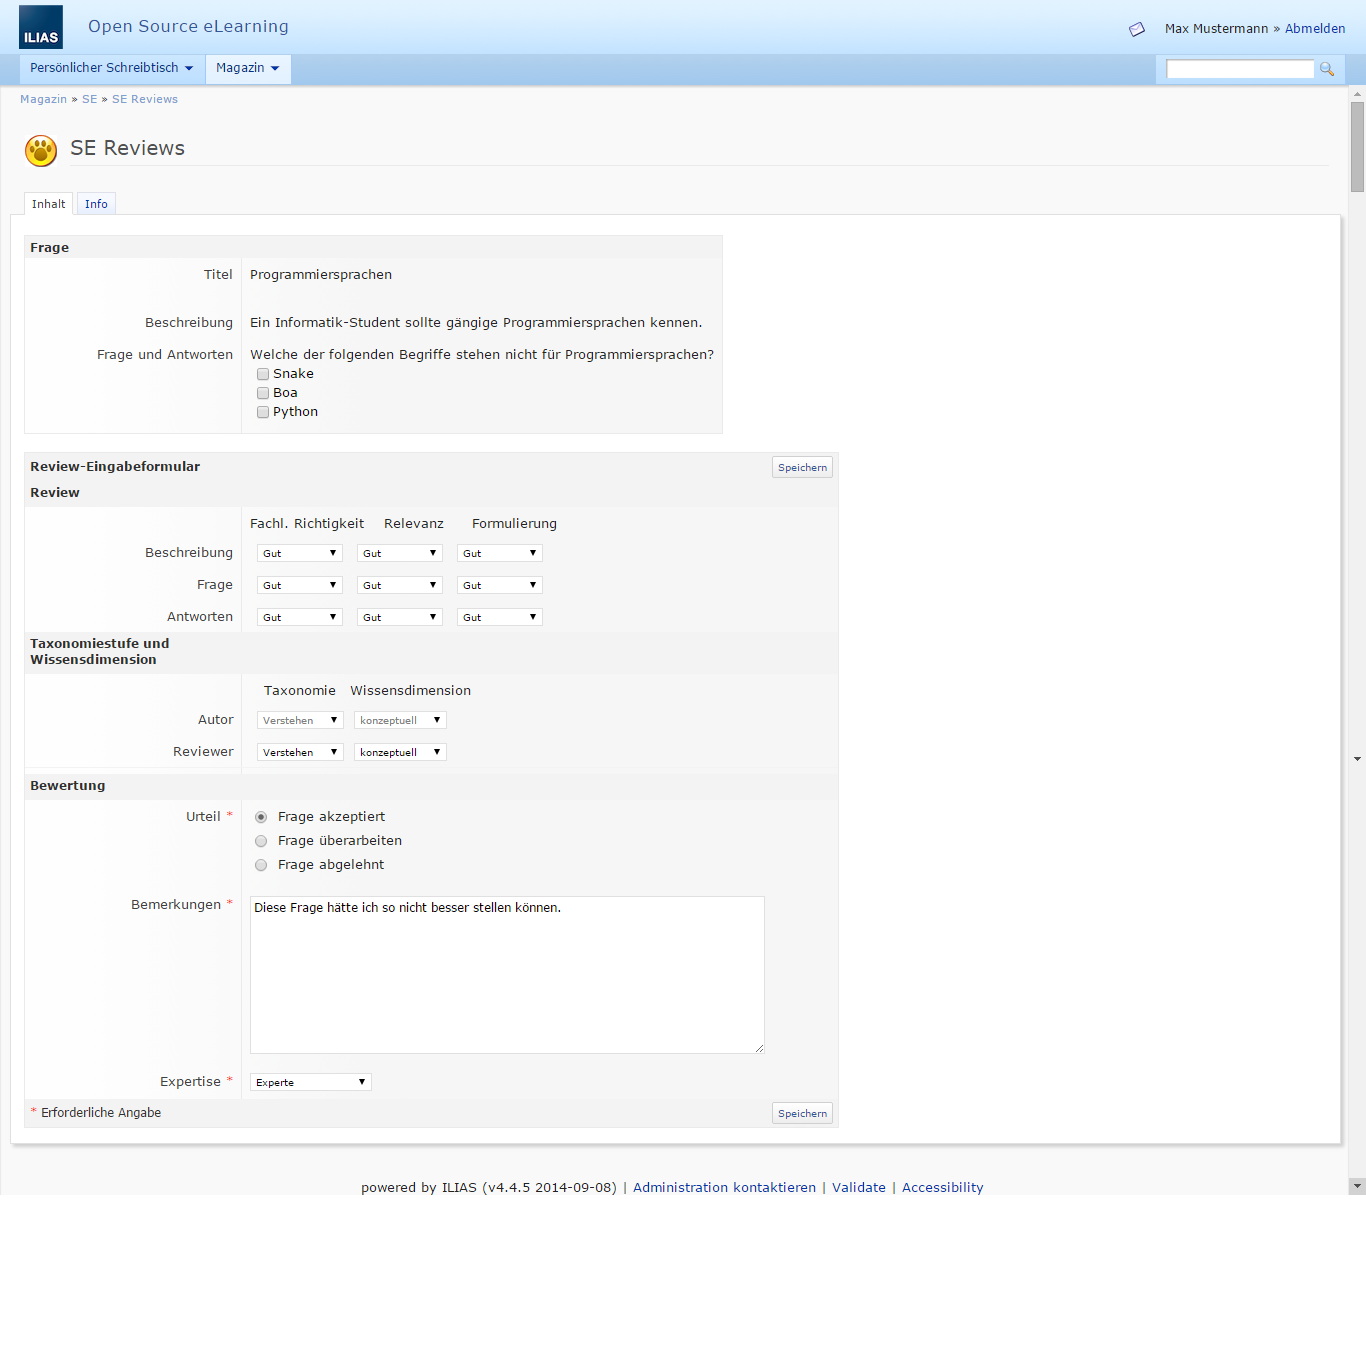
\includegraphics[width=1.0\textwidth]{reviewformular.png}

\section{Reviewansicht}
Die Seite sieht der zum Erstellen von Reviews sehr ähnlich. Der einzige Unterschied ist, dass die eingetragenen Werte nicht mehr zu bearbeiten sind. Es ist ebenfalls eine Fragenansicht sichtbar, sowie  eine Reihe an Dropdown-Listen und das Bemerkungsfeld. \\
\\
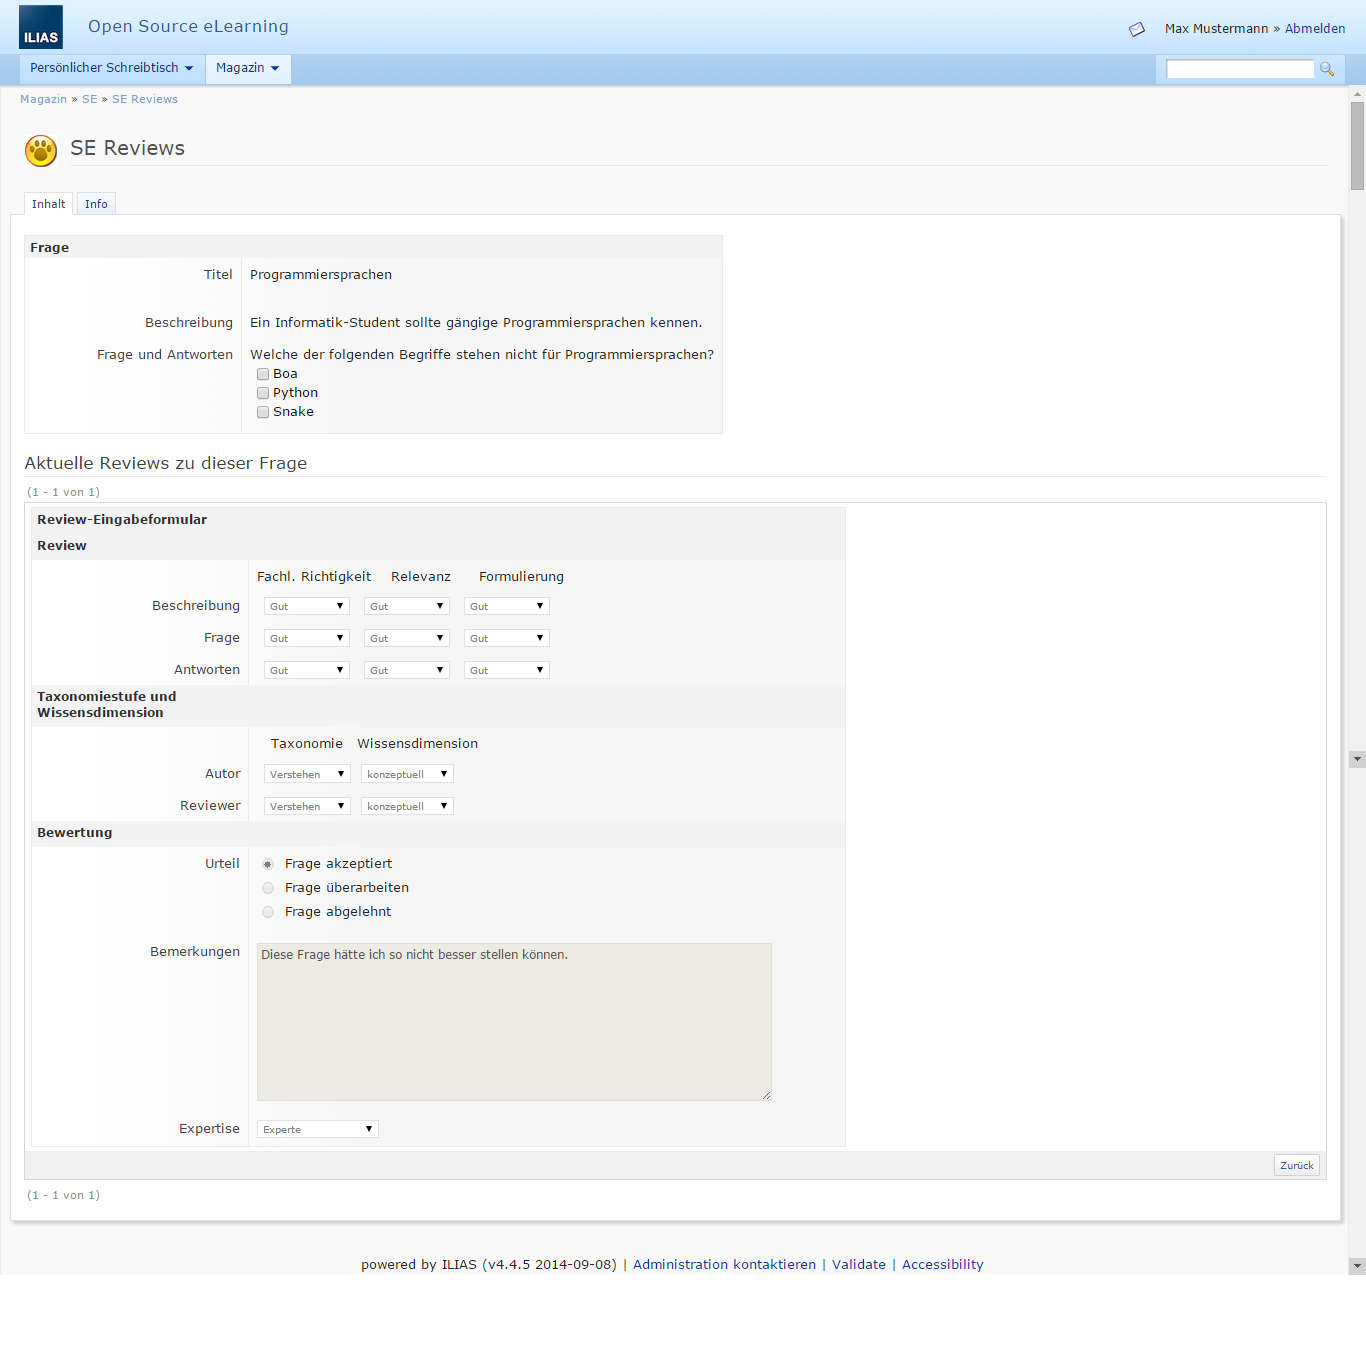
\includegraphics[width=1.0\textwidth]{reviewausgabe.png}

\section{Reviewer Zuordnungsseite}
Diese Seite ist dem Administrator bestimmt. Zu sehen ist eine Tabelle, in der horizontal alle Mitglieder dieser Gruppe und vertikal alle zu reviewenden Fragen gelistet sind. Um die Fragen Gruppenmitgliedern zuzuordnen, müssen die Checkboxen entsprechender Zeile und Spalte angeklickt werden. \\
\\
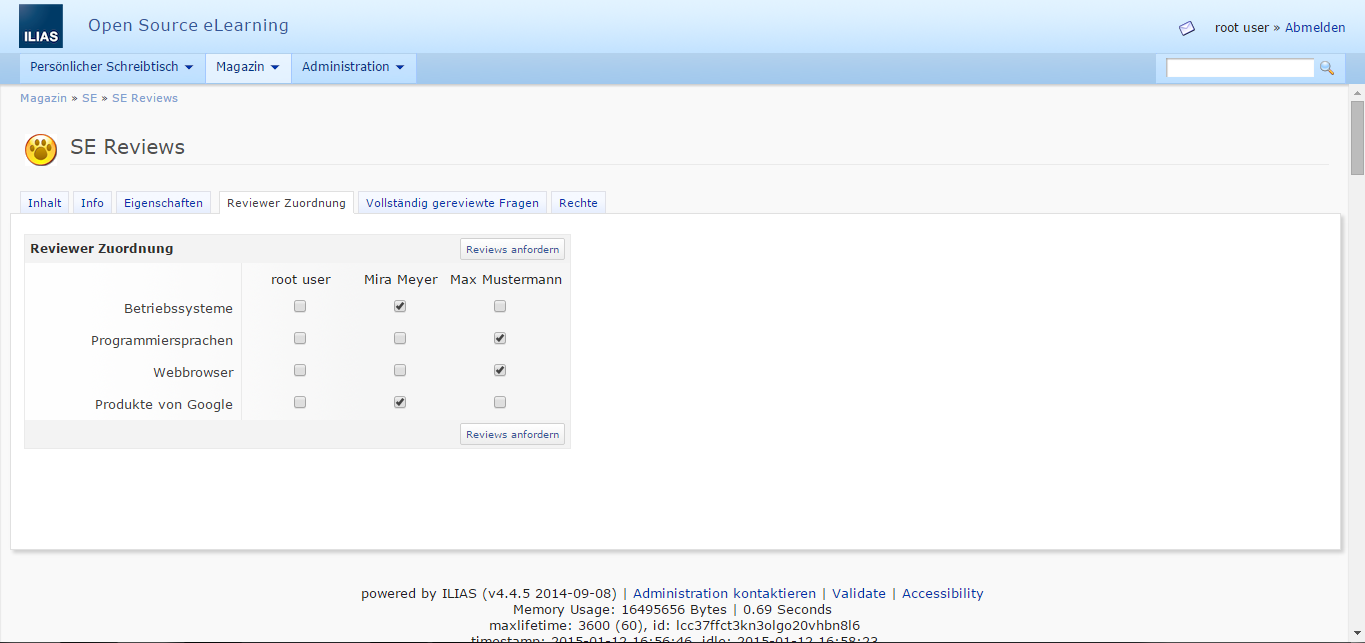
\includegraphics[width=1.0\textwidth]{reviewer_zuordnen.png}

\section{Übersicht vollständig gereviewter Fragen}
Hier werden alle fertig gereviewten Fragen gelistet, damit ein Administrator sie freischalten kann. Die freigegebenen Fragen sind dann für die Verwendung in Tests geeignet. \\
\\
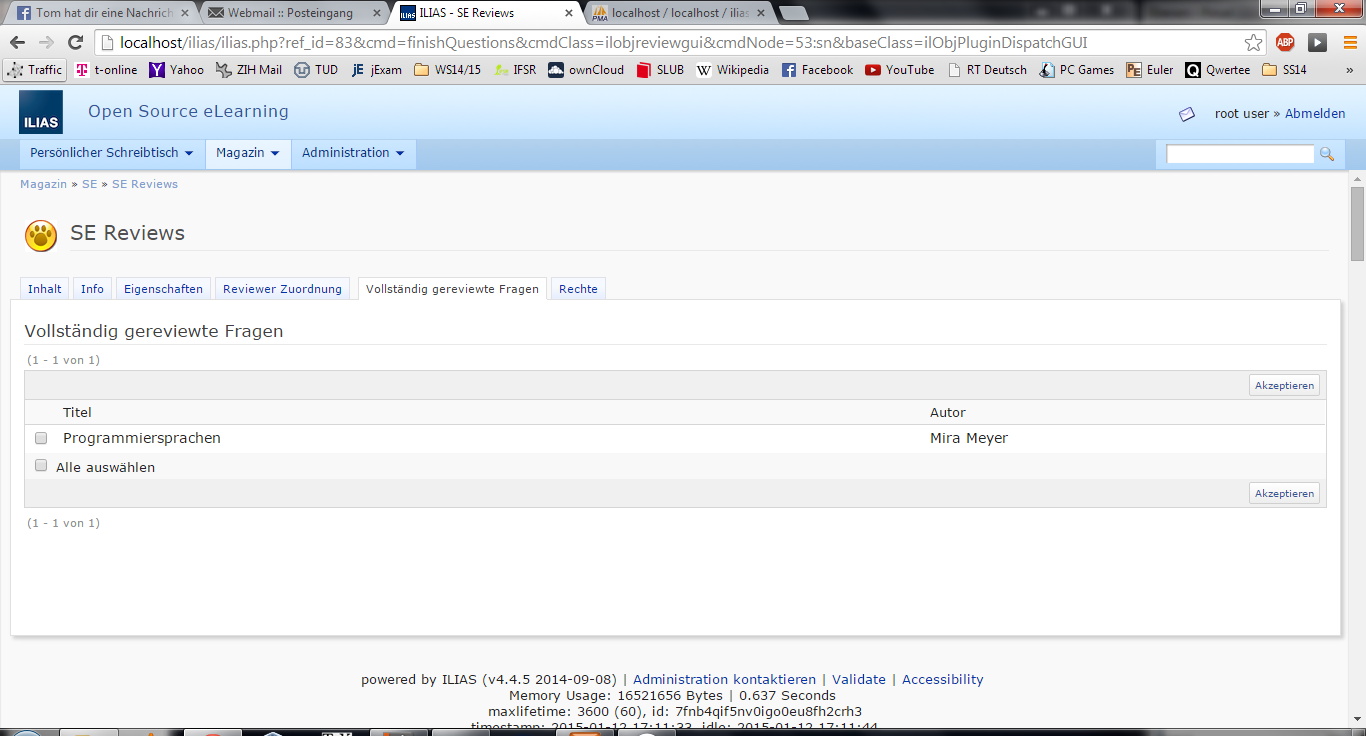
\includegraphics[width=1.0\textwidth]{frage_fertigstellen.png}

\chapter{Sie sind eingeloggt}

\section{als Administrator}
	
\subsection{Reviewpool erstellen}
Reviewpools werden in Gruppen erstellt. Neben dem Reviewpool muss ein Fragenpool existieren, denn für Reviews sind reviewbare Fragen notwendig. Um einen Reviewpool zu erstellen klicken Sie auf den grünen Button 'Neues Objekt hinzuf"ugen'. Eine Übersicht öffnet sich. Wählen Sie ganz rechts unten unter 'Weitere' Review aus. Eine Seite öffnet sich, die Sie um einen Titel und eine Beschreibung für das Review-Objekt fragt. Füllen sie beides aus und klicken sie final auf 'Review hinzufügen'.
		
\subsection{Reviews zuteilen}
Wählen Sie über 'Magazin' Ihren Reviewpool aus und betreten Sie ihn. Wechseln Sie nun von dem Reiter 'Inhalt' zu 'Reviewer Zuordnung'. Wählen Sie in der Tabelle die Checkboxen mit den passenden Zeilen und Spalten an und klicken Sie auf 'Reviews anfordern' um die Reviewer zu benachrichtigen und Ihre Einstellung zu speichern.
		
\subsection{Vollständige Reviews freigeben}
Wählen Sie über 'Magazin' Ihren Reviewpool aus und betreten Sie ihn. Wechseln Sie nun von dem Reiter 'Inhalt' zu 'Vollst"andig gereviewte Fragen'. W"ahlen Sie in der Liste der fertig gereviewten Fragen die Fragen, die Sie freigeben m"ochten an und klicken Sie rechts auf den Button 'Akzeptieren'. Die Fragen erscheinen von nun an nicht mehr im Reviewpool und sind für die Erstellung von Tests geeignet.
		
\subsection{Eigenschaften des Reviewpools bearbeiten}
Wählen Sie über 'Magazin' Ihren Reviewpool aus und betreten Sie ihn. Wechseln Sie nun von dem Reiter 'Inhalt' zu 'Eigenschaften'. Bearbeiten Sie gegebenenfalls Titel und Beschreibung des Reviewpools und klicken auf 'Speichern'. 
		
\subsection{Rechte bearbeiten}
Wählen Sie über 'Magazin' Ihren Reviewpool aus und betreten Sie ihn. Wechseln Sie nun von dem Reiter 'Inhalt' zu 'Rechte'. Mit einem Dropdown-Feld können Sie die Rollen auswählen, für die die Rechte bearbeitet werden sollen. In der Tabelle darunter können Sie den ausgewählten Rollen Berechtigungen durch das Anklicken von Checkboxen verteilen. Klicken Sie auf 'Speichern', um Ihre Einstellungen festzusetzen. 
		
\section{als Nutzer}
	
\subsection{Review erstellen}
Wählen Sie über 'Magazin' Ihren Reviewpool aus und betreten Sie ihn. Um ein Review erstellen zu können, muss vorher eine reviewbare Frage erstellt worden sein. Wenn Ihnen Fragen zum Reviewen zugeteilt werden, dann erreichen Sie das entsprechende Review-Eingabeformular in der unteren Tabelle namens 'Meine Reviews'. Klicken Sie auf Review erstellen, füllen Sie die Seite aus und speichern Sie es. \\		
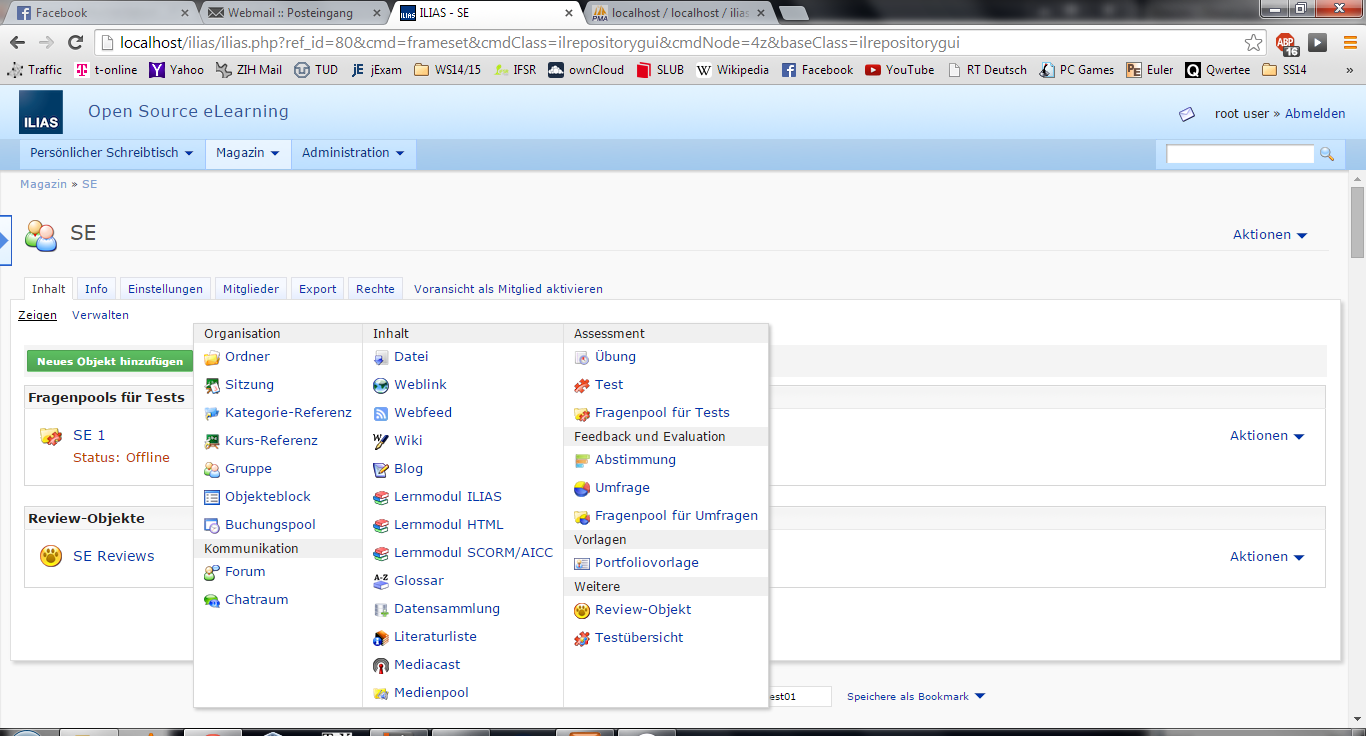
\includegraphics[width=1.0\textwidth]{reviewpool_erstellen.png}
		
\subsection{Frage erstellen}
Wählen Sie über 'Magazin' Ihren Fragenpool aus und betreten Sie ihn. Unter der Reiterleiste finden Sie den Button 'Frage erstellen'. Folgen Sie ihm und wählen Sie auf der folgenden Seite beispielsweise 'Multiple Choice (Reviewbar)', für eine Multiple Choice Frage. Klicken Sie auf 'Erstellen' und füllen Sie die folgende Seite aus. Der Prozess sieht dem üblichen Frageerstellungsprozess von ILIAS sehr ähnlich. 
		
\subsection{Review einsehen}
Wählen Sie über 'Magazin' Ihren Reviewpool aus und betreten Sie ihn. Falls Sie bereits Reviews verfasst haben sollten, so finden Sie sie in der unteren Tabelle namens 'Meine Reviews'. Klicken Sie auf 'Reviews einsehen', um Ihr Review und bereits erstellte Reviews anderer Gruppenmitglieder zu einer Frage anzuzeigen. Wollen Sie jedoch Reviews zu von Ihnen gestellten Fragen einsehen, so finden Sie diese in der oberen Tabelle namens 'Meine Fragen'. Nach einem Klick auf 'Reviews einsehen' werden alle aktuellen Reviews zu Ihrer Frage angezeigt.
		
\subsection{Frage exportieren}
Wählen Sie über 'Magazin' Ihren Fragenpool aus und betreten Sie ihn. Anschließend wählen Sie die Checkboxen der zu exportierenden Fragen aus. Wählen Sie aus der Dropdown-liste 'Exportieren' aus und klicken Sie auf 'Ausführen'. Der Download eines ZIP-Archivs sollte Ihnen angeboten werden. Speichern Sie dieses.
		
\subsection{Frage importieren}
Wählen Sie über 'Magazin' Ihren Fragenpool aus und betreten Sie ihn. Klicken Sie auf 'Importieren' rechts an der Seite bei der Auflistung von Fragen im Pool. Übergeben Sie ILIAS eine valide Datei. 
\end{document}